\documentclass[12pt,a4paper,utf8]{ctexart}
\usepackage{graphicx}
\usepackage{subfigure}
\usepackage{amsmath}
\usepackage{amssymb}
\usepackage{subfig}
\usepackage{cite}
\usepackage[ntheorem]{empheq}
\usepackage{enumitem}
\usepackage{fullpage}
\usepackage{cleveref}
\usepackage{cellspace}
\usepackage{listings}
\usepackage{color}

\usepackage{setspace}%使用间bai距宏包

\definecolor{gray}{rgb}{0.5,0.5,0.5}
\definecolor{dkgreen}{rgb}{.068,.578,.068}
\definecolor{dkpurple}{rgb}{.320,.064,.680}

% set Matlab styles
\lstset{
   language=Matlab,
   keywords={break,case,catch,continue,else,elseif,end,for,function,
      global,if,otherwise,persistent,return,switch,try,while},
   basicstyle=\ttfamily,
   keywordstyle=\color{blue}\bfseries,
   commentstyle=\color{dkgreen},
   stringstyle=\color{dkpurple},
   backgroundcolor=\color{white},
   tabsize=4,
   showspaces=false,
   showstringspaces=false
}

\begin{document}
\CJKfamily{zhkai}	



\begin{center}

   \begin{spacing}{2.0}%%行间距变为double-space
      \textbf{\heiti{\zihao {-1} 计算方法  作业一}}\\
   \end{spacing}

\textbf{姓名 \quad 龚小航 \qquad  学号 \quad PB18151866  \qquad 日期\quad 2020.10.18}\\
\end{center}
%\textit{}
%\vspace{\baselineskip}

\begin{enumerate}
\item[第一题] \textbf{重心插值公式(barycentric interpolation formula)}  

  \begin{enumerate}
    \item[$a)$] 用节点多项式
        \begin{equation}
           \ell(x)=\prod_{k=0}^n(x-x_{k})
        \end{equation}
    表示Lagrange插值基函数:\\
    先写出拉格朗日插值基函数以及节点多项式的导数在$x=x_j$处的值:
        \begin{equation}
           \ell_{j}(x)=\frac{\prod_{k \neq j}\left(x-x_{k}\right)}{\prod_{k \neq j}\left(x_{j}-x_{k}\right)} ;\label{cardinal}
           \quad  \quad \ell^{'}(x_j)=\frac{d}{dx}\ell (x)_{x=x_{j}}=\prod_{k \neq j}\left(x_{j}-x_{k}\right)
        \end{equation}
    对比发现恰好$\ell^{'}(x_j)$就是拉格朗日插值基函数的分母。由此可得它们的关系:
        \begin{equation}
            \ell_{j}(x)=\frac{\prod_{k \neq j}\left(x-x_{k}\right)}{\prod_{k \neq j}\left(x_{j}-x_{k}\right)} 
            =\frac{\prod_{k \neq j}\left(x-x_{k}\right)}{\ell^{'}(x_j)}
            =\frac{\ell(x)}{\ell^{'}(x_j)(x-x_{j})}
        \end{equation}
    由此可以推导出重心插值公式的第一形式:
        \begin{equation}
            p(x) = \sum_{j=0}^{n} f_j \ell_j(x)
            =\sum_{j=0}^{n} \frac{\ell(x)}{\ell^{'}(x_j)(x-x_{j})}f_j
            =\ell(x)\sum_{j=0}^{n} \frac{\lambda_{j}}{(x-x_{j})}f_j
        \end{equation}
    其中利用了替换$\lambda_{j}=1/\ell^{'}(x_j)$,$\lambda_{j}$称为插值权重。
    
    
    \item[$b)$] 证明所有的Lagrange插值基函数的和为1:\\
        观察公式$(1)$的形式,可取被插函数$f(x)=1$ ,在这个函数上
        插值,无论选取几个插值点,都有:
        \begin{equation}
            p(x) = \sum_{j=0}^{n} f_j \ell_j(x) = \sum_{j=0}^{n}\ell_j(x)=1
        \end{equation}
        这是由于$n$次插值多项式的误差为:
        \begin{equation}
            R_{n}(x) = \frac{f^{(n+1)}(\xi)}{(n+1)!}\prod_{i=0}^{n}(x-x_{i})=0 
        \end{equation}
        由于$f$是常数,一阶及以上的导数都为$0$。\\
        再由此推出重心插值公式的第二形式:
        \begin{eqnarray} 
            p(x) &=& \sum_{j=0}^{n} f_j \ell_j(x) = \sum_{j=0}^{n} f_j \frac{\prod_{k \neq j}\left(x-x_{k}\right)}{\prod_{k \neq j}\left(x_{j}-x_{k}\right)}\nonumber \\ 
                 &=& \prod_{i=0}^{n}(x-x_{i})\sum_{j=0}^{n}\frac{f_j}{(x-x_{j})\prod_{k \neq j}\left(x_{j}-x_{k}\right)}                                    \nonumber \\ 
                 &=& \frac{\prod_{i=0}^{n}(x-x_{i})\sum_{j=0}^{n}\frac{f_{j}\lambda_{j}}{(x-x_{j})}}{\sum_{j=0}^{n}\ell_j(x)}
                  =  \frac{\sum_{j=0}^{n}\frac{f_{j}\lambda_{j}}{(x-x_{j})}}{\sum_{j=0}^{n}\frac{\prod_{k \neq j}(x-x_{k})}{\prod_{i=0}^{n}(x-x_{i})\prod_{k \neq j}(x_{j}-x_{k})}} \nonumber \\
                 &=& \frac{\sum_{j=0}^{n}\frac{f_{j}\lambda_{j}}{(x-x_{j})}}{\sum_{j=0}^{n}\frac{1}{(x-x_{j})\prod_{k \neq j}(x_{j}-x_{k})}} \nonumber \\
                 &=& \frac{\sum_{j=0}^{n}\frac{f_{j}\lambda_{j}}{(x-x_{j})}}{\sum_{j=0}^{n}\frac{\lambda_{j}}{(x-x_{j})}}
        \end{eqnarray}
    \item[$c)$] 即需要证明的是:\\
        \begin{eqnarray}
            x_{j}=cos(\frac{j\pi}{n}),j=0,1,2,···,n  \\
            \prod_{k=0,k!=j}^{n}\frac{1}{x_{j}-x_{k}}=
            \left\{\begin{array}{ll}
                \frac{2^{n-2}}{n} & j=0 \\
                \frac{2^{n-1}}{n}(-1)^{j} & 0<j<n \\
                \frac{2^{n-2}}{n}(-1)^{n} & j=n \\
                \end{array}\right. \nonumber
        \end{eqnarray}
        \quad \quad 为证明这个关系式,由结果的特点,可以利用数学归纳法。证明$j=j和j=j+1$
        之间的关系即可:\\
        先计算$j=0$的情况:$x_{0}=cos(0)=1$\\
        \begin{eqnarray}
            \prod_{k=1}^n(1-cos\frac{k\pi}{n}) &=& \prod_{k=1}^{n-1}(sin^{2}\frac{k\pi}{2n})=\prod_{k=1}^{n-1}(sin\frac{k\pi}{2n}cos\frac{(n-k)\pi}{2n}) \\
            &=&\prod_{k=1}^{n-1} cos(\frac{k\pi}{2n})sin(\frac{(n-k)\pi}{2n}) \quad (k\Rightarrow n-k) \\
            &=&(\prod_{k=1}^{n-1} cos(\frac{k\pi}{2n})sin(\frac{k\pi}{2n})cos(\frac{(n-k)\pi}{2n})sin(\frac{(n-k)\pi}{2n}))^\frac{1}{2} \\
            &=&\frac{1}{2^{n-1}} \prod_{k=1}^{n-1}sin(\frac{k\pi}{n})
        \end{eqnarray}
        \quad \quad 再计算这个求和式:
        
        \begin{eqnarray}
           \prod_{k=1}^{n-1} sin(\frac{k\pi}{n}) &=& \prod_{k=1}^{n-1}(\frac{e^{\frac{ik\pi}{n}}-e^{\frac{-ik\pi}{n}}}{2i})=\frac{1}{(2i)^{n-1}}\prod_{k=1}^{n-1}(e^{\frac{ik\pi}{n}}-e^{\frac{-ik\pi}{n}}) \\
            &=& \frac{1}{(2i)^{n-1}}(\prod_{k=1}^{n-1}e^{\frac{-ik\pi}{n}})(\prod_{k=1}^{n-1}(e^{\frac{2ik\pi}{n}}-1)) \\
            &=& \frac{1}{(2i)^{n-1}}e^{-i\frac{(n-1)\pi}{2}}\prod_{k=1}^{n-1}(\xi ^{k}-1) \\
                (f(x) &=& \prod_{k=1}^{n-1}(x-\xi^k)=\frac{x^n-1}{x-1}=\Sigma _{k=0}^{n-1}\xi ^{k}) \\
            &=& \frac{1}{(2i)^{n-1}}e^{-i\frac{(n-1)\pi}{2}}(-1)^{n-1}*n  \\
            &=& \frac{n}{2^{n-1}} \\
            \Longrightarrow  \prod_{k=1}^{n}\frac{1}{1-cos(\frac{k\pi}{n})}=\frac{2^{n-2}}{n}

        \end{eqnarray}
        再计算其递推式:\\
        即需要证明$j=j+1$时与$j=j$时相比仅多出一个负号。\\
            \\
            \quad \quad 未证完整
            \\
            \\
            \\
            \\
            \\
            \\
            \\
            \\
            \\
            \\
            \\



    \item[$d)$] 代码如下所示:
    \begin{lstlisting}[frame=single]
    clear, clc, clf
    LW = 'linewidth'; lw = 2;
    format long;
    
    n = 5000;
    x = zeros(1,5001);
    for i=1:n+1
       x(i) = cos((i-1)*pi/n); 
    end
    F = @(x) tanh(20.*sin(12.*x))+0.02.*exp(3.*x)
             .*sin(300.*x);
    f = F(x);
    
    figure(1)
    plot(x,F(x));
    title('以5001切比雪夫点为插值点做出的被插函数图像')
    xlabel('x')
    ylabel('f(x)')
    
    
    t = linspace(-1, 1, 2*n+1)';
    vart=check(t);
    
    figure(2)
    plot(t,vart);
    title('对10001个等距点利用重心插值公式得到的p(x)图像')
    xlabel('x')
    ylabel('p(x)')
    
    figure(3)
    semilogy(t,abs(vart-F(t)));
    title('10001个点的|F(x)-p(x)|')
    xlabel('x')
    ylabel('log R')
    
    function G = check(t)   %%做出10001个点得到的p(x)
    i = 1;
        n = 5000;
       x = zeros(1,5001);
       for i=1:n+1
         x(i) = cos((i-1)*pi/n); 
       end
       F = @(x) tanh(20.*sin(12.*x))+0.02.*exp(3.*x)
                .*sin(300.*x);
    
        r1=(-F(x(1))./(t-x(1)))./2+((-1).^(n+1)
           .*F(x(n+1))./(t-x(n+1)))./2;
        r2=((-1)./(t-x(1)))./2+((-1).^(n+1)
            ./(t-x(n+1)))./2;
        for i = 2 : n 
             r1=r1+(((-1).^i.*F(x(i))./(t-x(i))));
             r2=r2+(((-1).^i./(t-x(i))));
        end
        G = r1./r2;  
    end

    \end{lstlisting}
    \quad \quad 由题意做出$5001$个切比雪夫点,将它们用作插值点构造标准函数
    $F(x)$,再在$[-1,1]$上均匀取$10001$个点作重心插值得到插值函数$p(x)$。
    最后做出$10001$个点与其误差组成的y轴半对数图。结果如下所示:\\
    \begin{figure}[htbp]
        \centering
        \subfigure[利用5001个切比雪夫插值点作出的原函数f(x)]{
        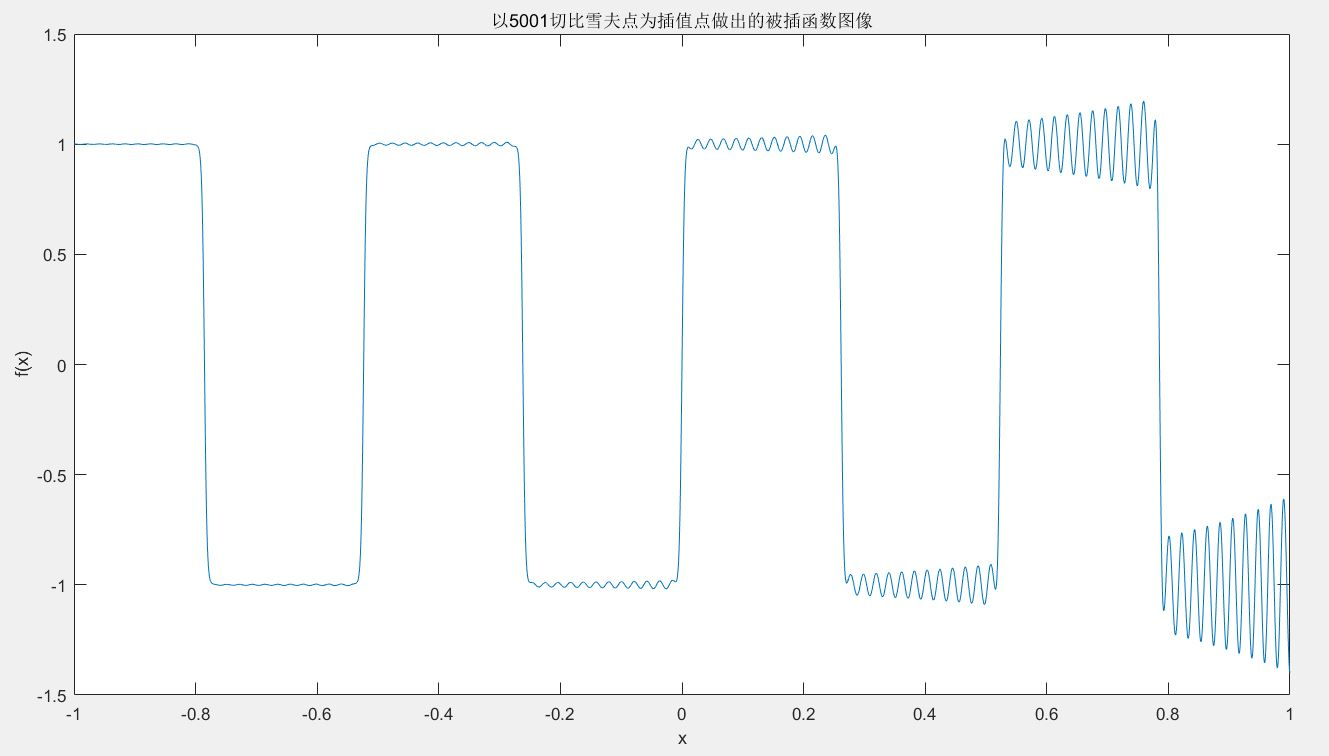
\includegraphics[width=9cm]{T3_5001.JPG}
        %\caption{fig1}
        }
        \quad
        \subfigure[用10001个等距点重心插值出的p(x)]{
        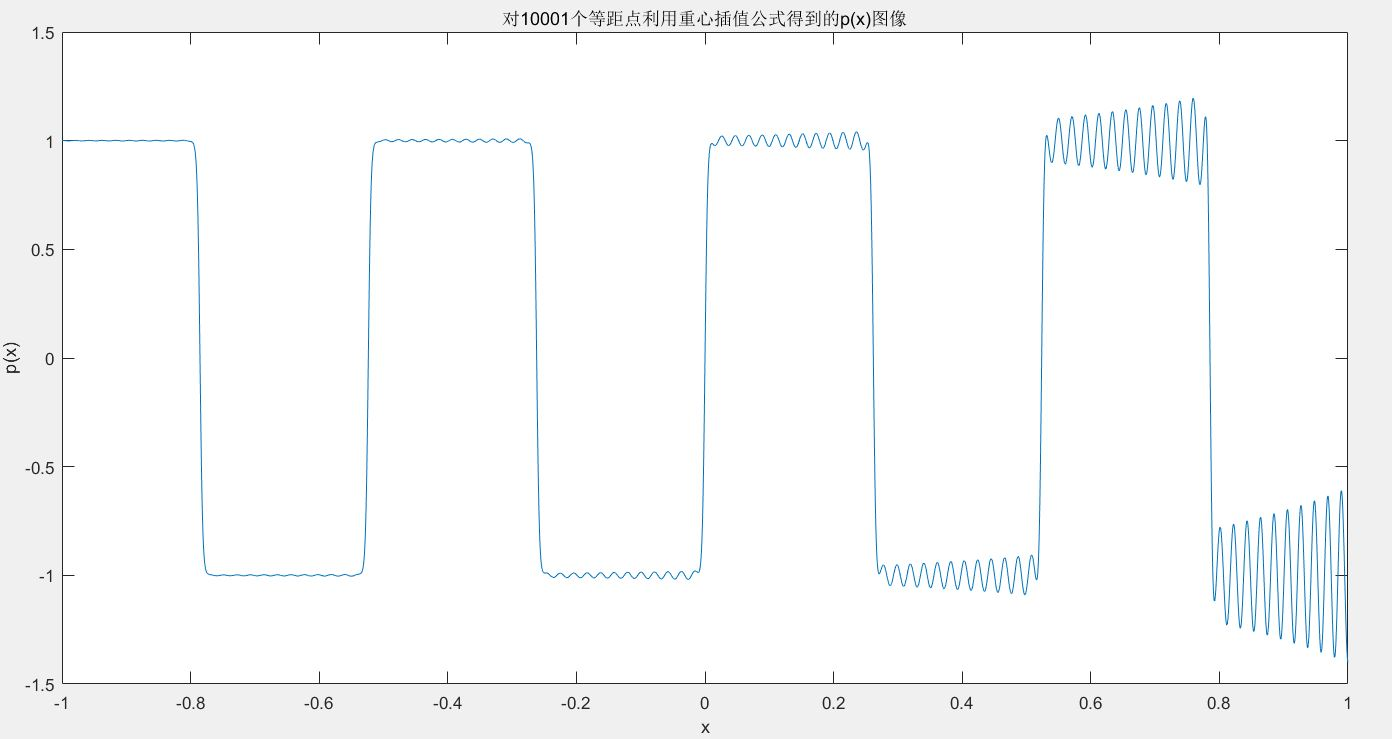
\includegraphics[width=9cm]{T3_10001.JPG}
        }
        \quad
        \subfigure[|p(x)-F(x)|]{
        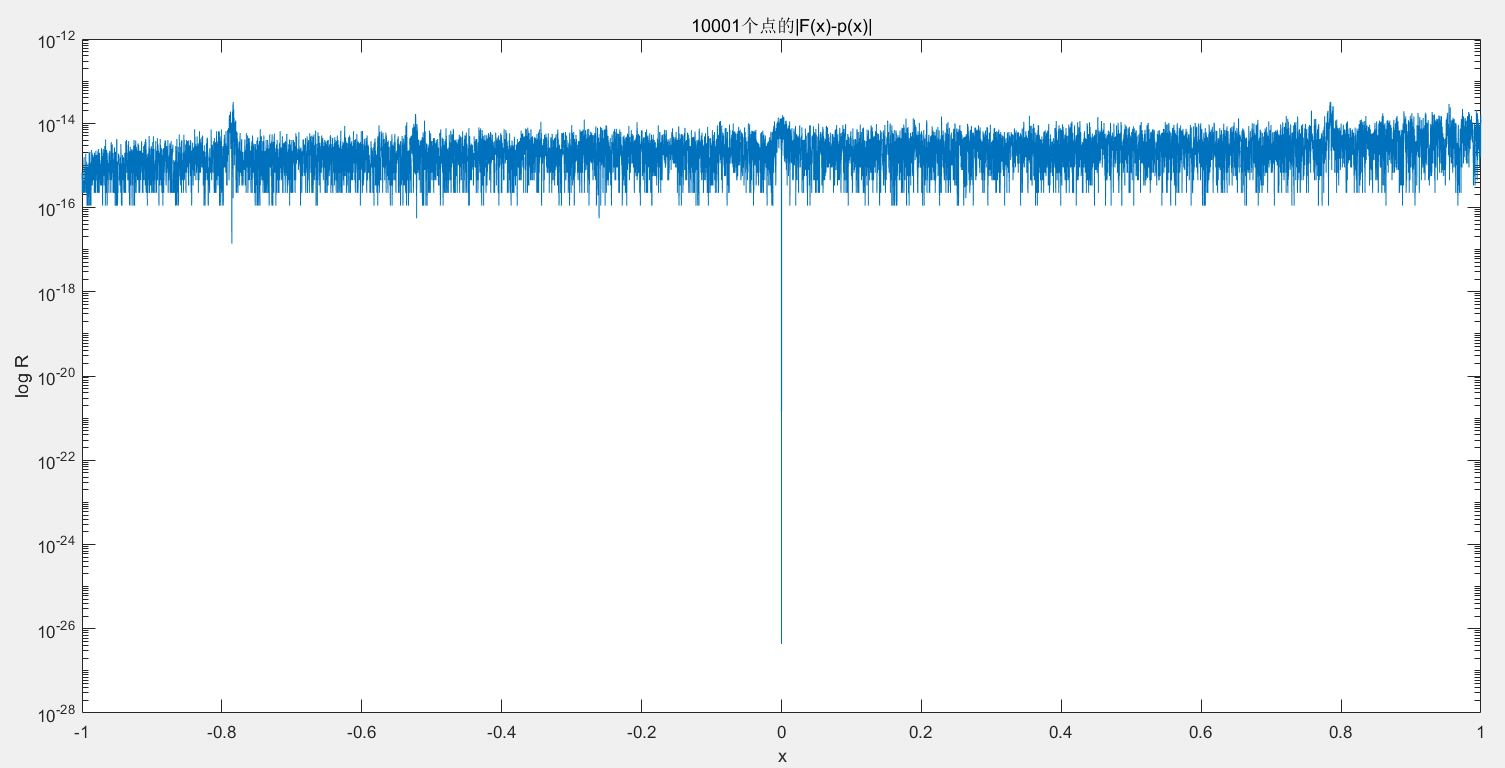
\includegraphics[width=9cm]{T3F_P.JPG}
        }
        
        \caption{第一题 d 问插图}
    \end{figure}
    \\
    \\
    \\
    \\
    \\
    \\
    \\
    \\
    \\
    \\
  \end{enumerate}
       


\item[第二题]
\textsc{Matlab}程序显示如下:
\begin{lstlisting}[frame=single]
    clear, clc, clf
    LW = 'linewidth'; lw = 2;
    format long;
    
    [p61,p62,p63]=T2(6);
    [p71,p72,p73]=T2(7);
    [p81,p82,p83]=T2(8);
    [p91,p92,p93]=T2(9);
    [p101,p102,p103]=T2(10);
    [p111,p112,p113]=T2(11);
    [p121,p122,p123]=T2(12);
    
    y1 = [p61,p71,p81,p91,p101,p111,p121];
    y2 = [p62,p72,p82,p92,p102,p112,p122];
    y3 = [p63,p73,p83,p93,p103,p113,p123];
    k = 6:1:12;
    x = 2.^k;
    
    figure(1)
    pic1=loglog(x,y1,'k');hold on
    pic2=loglog(x,y2,'g');hold on
    pic3=loglog(x,y3,'r');hold on
    legend([pic1,pic2,pic3], '第一类边界条件', 
            '第二类边界条件','第三类边界条件')
    title('第二题误差图')
    xlabel('log n')
    ylabel('log max{|S-F(x)|}')
    
    
    function [p1,p2,p3]=T2(k)    
        n = 2^k;
        
    x = linspace(-1, 1, n+1)';
    F = @(x) exp(3.*cos(pi.*x));
    f = F(x);
    %%
    h = diff(x);
    df = diff(f);
    lambda = h(2:n) ./ (h(2:n) + h(1:n-1));
    d = 6 * ( df(2:n) ./ h(2:n) - df(1:n-1) 
        ./ h(1:n-1) ) ./ (h(2:n) + h(1:n-1));
    mu = 1-lambda;
    %%
    %第一类边界条件
    M0 = 0;
    Mn = 0;
    A1 = diag(2*ones(n-1,1)) + diag(lambda(1:n-2), 1) 
         + diag(mu(2:n-1), -1);
    D1 = [d(1) - mu(1)*M0; d(2:n-2); d(n-1) 
        - lambda(n-1)*Mn];
    M1 = A1\D1;
    M1 = [M0; M1; Mn];
    %%
    %第二类边界条件
    m0 = 0;
    mn = 0;
    lambda2 = [1; lambda];
    mu2 = [mu; 1];
    d0 = 6 * ( df(1) / h(1) - m0 ) / h(1);
    dn = 6 * ( mn - df(n) / h(n) ) / h(n);
    D2 = [d0; d; dn];
    A2 = diag(2*ones(n+1,1)) + diag(lambda2, 1) 
         + diag(mu2, -1);
    M2 = A2\D2;
    %%
    %第三类边界条件
    lambda0 = h(1) / (h(1) + h(n));
    lambda3 = [lambda0; lambda(1:n-2)];
    mu0 = 1 - lambda0;
    d0 = 6 * (df(1) ./ h(1) - df(n) ./ h(n)) 
         / (h(1) + h(n));
    D3 = [d0; d];
    A3 = diag(2*ones(n,1)) + diag(lambda3, 1) 
         + diag(mu, -1);
    A3(1, n) = mu0;
    A3(n, 1) = lambda(n-1);
    M3 = A3\D3;
    M3 = [M3; M3(1)];
    
    %%
    p1 = CubicSpline(x, F, h, M1);
    %display(p1);
    
    p2 = CubicSpline(x, F, h, M2);
    %display(p2);
    
    p3 = CubicSpline(x, F, h, M3);
    %display(p3);
    end
    
    
    function result = CubicSpline(x, F, h, M)
    n = size(x) - 1;
    f = F(x);
    result = 0;
    for k = 1:n
        m = 6;
        xx = linspace(x(k), x(k+1), m)';
        S = ( (x(k+1)-xx).^3*M(k) + (xx-x(k)).^3*M(k+1) ) 
            / (6*h(k)) +( (x(k+1)-xx)*f(k) 
            + (xx-x(k))*f(k+1) ) 
            / h(k) -h(k) * ( (x(k+1)-xx)*M(k) 
            + (xx-x(k))*M(k+1) ) / 6;
        
        resulti=max(abs(S-F(xx)));
        if(resulti>result)
            result=resulti;
        end
    end
        
    end
    
\end{lstlisting}
    \quad \quad 本题可以通过自定义函数,通过输入$k$的值来确定在一、二、三类边界
    条件下$[x_[k],x_{k+1}]$上误差的最大值并返回三个值。在函数外的脚本主体部分
    比较简单,只负责将$k=6:1:12$时函数的返回值都储存在一个变量内,再将其作与$n$
    的关系图即可。脚本运行结果如下图所示:
    \begin{figure}[h]
        \centering
        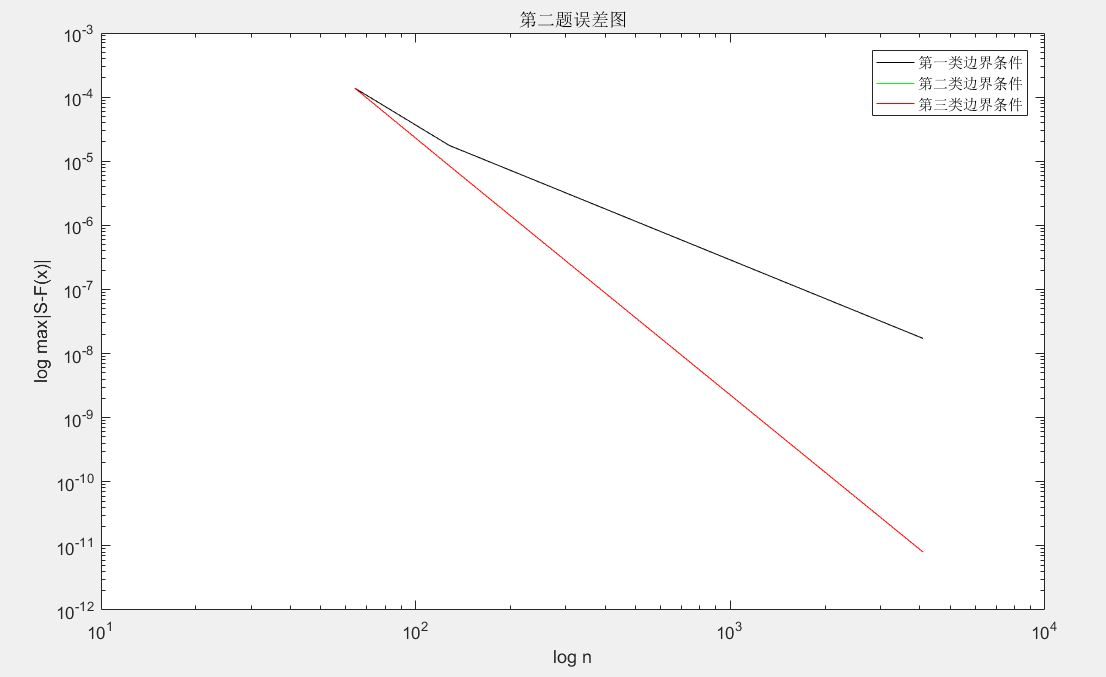
\includegraphics[width=1\textwidth]{第二题误差图.JPG}
        \caption{第二题误差图}
    \end{figure}\\
    \quad \quad 其中第二类和第三类边界条件下误差差值不是非常明显。在这幅图中,
    线的斜率表示当n的规模以$2^n$增大时,误差随插值点规模减小的速率。
    \\
    \\
    \\
    \\
    \\




\item[第三题]  \quad  对下列数据进行形如$y=ae^{bx}$形式的最小二乘拟合:\\
    \begin{table}[htbp]
    \centering
    \begin{tabular}{ccccc}%l=left, r=right,c=center分别代表左对齐,右对齐和居中,字母的个数代表列数
    \hline
    $x_{i}$ &$-0.70$ & $-0.50$  & $0.25$  & $0.75$  \\ \hline
    $y_{i}$ &$0.99$  & $1.21$   & $2.57$  & $4.23$  \\ \hline
    \end{tabular}
    \end{table}
    
    \quad \quad 由课本53页的例子,多项式拟合的方法可以推广到其他类型的函数拟合。对于本题中的
    形式$y=ae^{bx}$,先对其取对数,令$\hat{y_{i}}=ln(y_i)$,然后对$(x_{i},\hat{y_{i}}),i=1,2,···,m$
    作形如$ln\varphi(x)=ln a+bx$的线性拟合。即求$c_{0}=ln a,c_{1}=b$使得
    $\hat{Q}(c_{0},c_{1})=\sum _{i=1}^{4}(c_{0}+c_{1}x_{i}-\hat{y_{i}})$达到最小值。\\
    \quad \quad 直接在matlab中调用函数解决这个线性拟合问题:\\

    \begin{figure}[h]
        \centering
        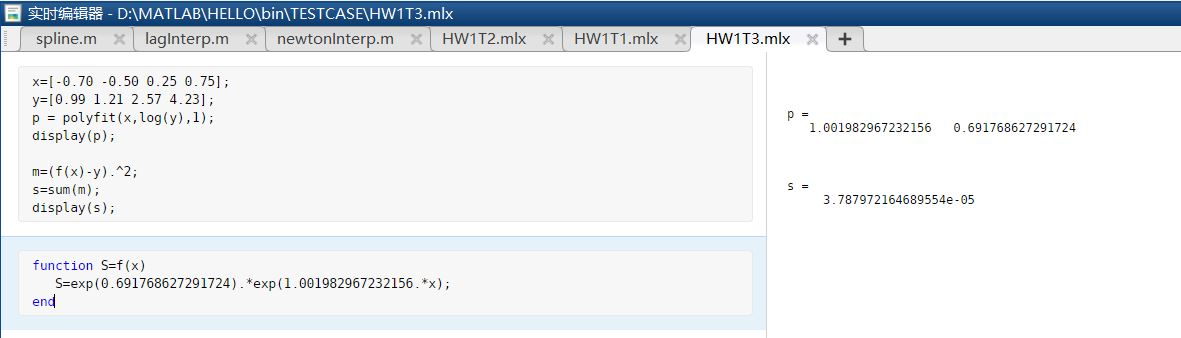
\includegraphics[width=1\textwidth]{T3.JPG}
        \caption{第三题求解代码}
    \end{figure}

    即得到结果$b=1.0020, ln a=0.6918 \Rightarrow a=1.9972$。即拟合结果为:
    \begin{equation}
        y=1.9972e^{1.0020x}
    \end{equation}
    \quad \quad 所得函数的误差2范数已在图中给出,为:
    \begin{equation}
        s=3.7880*10^{-5}
    \end{equation}





\end{enumerate}




\end{document}
